\chapter{Mode~S enhanced surveillance}

Mode~S Enhanced Surveillance (EHS) provides a set of advanced functionalities for the Mode~S transponders. Three different types of reports are included in EHS. They are designed to report vertical intent, turning performance, and airspeeds. This chapter explaines structures and decoding processes of these reports.

\section{Selected vertical intention (BDS 4,0)}

The selected vertical intention message is designed for air traffic control to obtain an aircraft's current vertical intentions. For example, an aircraft controller can use this information to check whether an aircraft is complying with an altitude command. Table \ref{tb:bds40} shows the structure of the message.

\begin{table}[ht]
\renewcommand{\arraystretch}{1.1}
\centering
\caption{Selected intention (BDS 4,0), MB field}
\label{tb:bds40}
\begin{tabular}{|l|l|l|l|}
\hline
\textbf{FIELD} & \textbf{MSG} & \textbf{MB} & \textbf{BITS} \\ \hline
Status (for MCP/FCU selected altitude) & 33 & 1 & 1 \\ \cdashline{1-4}
MCP/FCU selected altitude & 34--45 & 2--13 & 12 \\
~~Range: {[}0, 65520{]} ft &&& \\
~~LSB: 16 ft &&& \\ \hline
Status (for FMS selected altitude) & 46 & 14 & 1 \\ \cdashline{1-4}
FMS selected altitude & 47--58 & 15--26 & 12 \\
~~Range: {[}0, 65520{]} ft &&&\\
~~LSB: 16 ft &&& \\ \hline
Status (for barometric press setting) & 59 & 27 & 1 \\ \cdashline{1-4}
Barometric pressure setting  & 60--71 & 28--39 & 12 \\
~~Note: actual value minus 800 mb &&& \\
~~Range: {[}0, 410{]} mb &&& \\
~~LSB: 0.1 mb &&& \\ \hline
Reserved (all zeros) & 72--79 & 40--47 & 8 \\ \hline
Status of MCP/FCU mode & 80 & 48 & 1 \\ \cdashline{1-4}
VNAV mode & 81 & 49 & 1 \\ \cdashline{1-4}
Alt hold mode & 82 & 50 & 1 \\ \cdashline{1-4}
Approach mode & 83 & 51 & 1 \\ \hline
Reserved (all zeros) & 84--85 & 52--53 & 2 \\ \hline
Status of target altitude source & 86 & 54 & 1 \\ \cdashline{1-4}
Target altitude source & 87--88 & 55--56 & 2 \\ \hline
\end{tabular}
\end{table}

Two different types of selected altitude fields are included in the message. Values in the \emph{MCP/FCU selected altitude} field are from the mode control panel or flight control unit. These are often inputs from the pilot. Values in \emph{FMS selected altitude} field are derived from the flight management system controlling the vertical profile, which often does not come from manual input. In practice, FMS selected altitude values are often empty or unusable. When it is presented, the value is mostly the same as MCP/FCU selected altitude.

The \emph{barometric pressure setting} value is the actual pressure in millibars (mb) subtracted by a constant of 800. If the actual value is below 800 mb (or above 1209 mb), the corresponding status bit (MB:27) is set to \0.

The last two bits in the MB field show the source of the target altitude. They have the following meaning:

\begin{verbatim}
  00: Unknown source
  01: Aircraft altitude
  10: FCU/MCP selected altitude
  11: FMS selected altitude
\end{verbatim}


Figure \ref{fig:bds40_example} illustrates an example of how to decode a BDS 4,0 message.

\begin{figure}[ht]
  \centering
  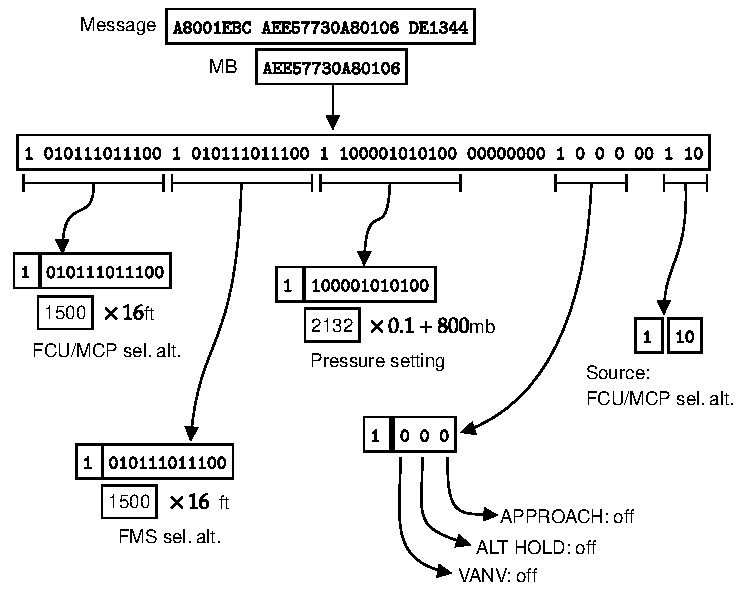
\includegraphics[scale=0.9]{figures/mode_s/bds40_example.pdf}
  \caption{BDS 4,0 decoding example}
  \label{fig:bds40_example}
\end{figure}

\begin{notebox}{Try it out}
Using pyModeS, we can decode information of BDS 4,0 messages as: 

\begin{verbatim}
import pyModeS as pms

msg = "A8001EBCAEE57730A80106DE1344"

pms.commb.selalt40fms(msg)
# 24000, FMS selected altitude (ft)

pms.commb.selalt40mcp(msg)
# 24000, MCP selected altitude (ft)

pms.commb.p40baro(msg)
# 1013.2, pressure (mb)
\end{verbatim}

\end{notebox}


\clearpage

\section{Track and turn report (BDS 5,0)}

The track and turn report is designed to provide parameters to describe aircraft turns. In this type of message, roll angle, track angle, and track rate are provided. It also includes the ground speed and true airspeed (TAS) of the aircraft.

Table \ref{tb:bds50} shows the structure of the message.

\begin{table}[ht]
\renewcommand{\arraystretch}{1.1}
\centering
\caption{Track and turn report (BDS 5,0), MB field}
\label{tb:bds50}
\begin{tabular}{|l|l|l|l|}
\hline
\textbf{FIELD} & \textbf{MSG} & \textbf{MB} & \textbf{BITS} \\ \hline
Status (for roll angle) & 33 & 1 & 1 \\ \cdashline{1-4}
Sign & 34 & 2 & 1 \\ \cdashline{1-4}
Roll angle & 35--43 & 3--11 & 9\\
~~Range: {[}-90, +90{]} degrees &&& \\
~~LSB: 45/256 degrees &&& \\ \hline
Status (for track angle) & 44 & 12 & 1 \\ \cdashline{1-4}
Sign & 45 & 13 & 1 \\ \cdashline{1-4}
True track angle & 46--55 & 14--23 & 10 \\
~~Range: {[}-180, 180{]} degrees &&& \\
~~LSB: 90/512 degrees &&& \\ \hline
Status (for ground speed) & 56 & 24 & 1 \\ \cdashline{1-4}
Ground speed & 57--66 & 25--34 & 10\\
~~Range: {[}0, 2046{]} kt &&& \\
~~LSB: 2 kt &&& \\ \hline
Status (for track angle rate) & 67 & 35 & 1 \\ \cdashline{1-4}
Sign & 68 & 36 & 1 \\ \cdashline{1-4}
Track angle rate & 69--77 & 37--45 & 9 \\
~~Range: {[}-16, 16{]} degrees/second &&& \\
~~LSB: 8/256 degrees/second &&& \\ \hline
Status (for true airspeed) & 78 & 46 & 1 \\ \cdashline{1-4}
True airspeed & 79--88 & 47--56 & 10 \\
~~Range: {[}0, 2046{]} kt &&& \\
~~LSB: 2 kt &&& \\ \hline
\end{tabular}
\end{table}

In this message, three signed values are shown, which are roll angle, track angle, and track angle rate. Two's complement coding (see section \ref{sec:two_complement}) should be used to calculate these values. 

The following Figure \ref{fig:bds50_example} shows an example of decoding a BDS 5,0 message.

\begin{figure}[ht]
  \centering
  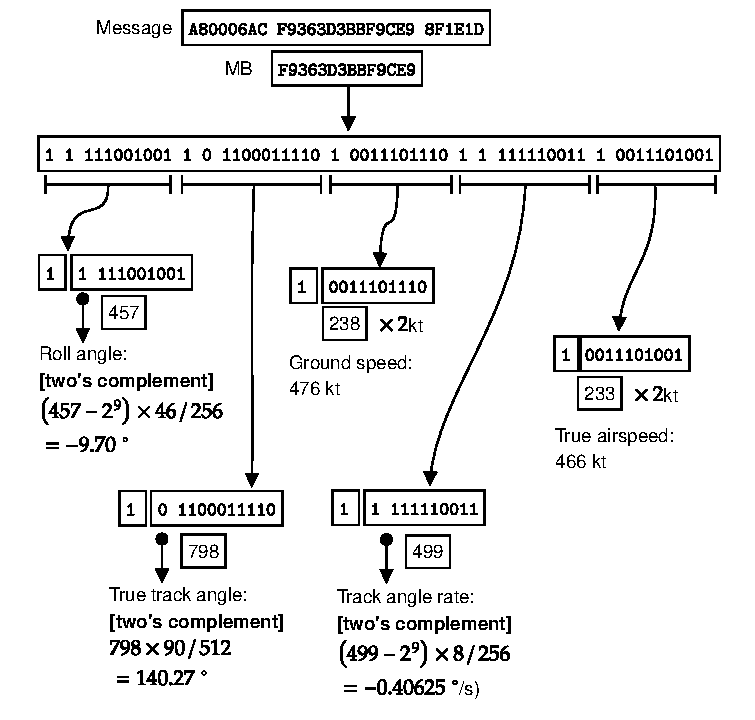
\includegraphics[scale=0.9]{figures/mode_s/bds50_example.pdf}
  \caption{BDS 5,0 decoding example}
  \label{fig:bds50_example}
\end{figure}

\begin{notebox}{Try it out}
Using pyModeS, we can decode information of BDS 5,0 messages as: 

\begin{verbatim}
import pyModeS as pms

msg = "A80006ACF9363D3BBF9CE98F1E1D"

pms.commb.roll50(msg)   # -9.7, roll angle (deg)
pms.commb.trk50(msg)    # 140.273, track angle (deg)
pms.commb.rtrk50(msg)   # -0.406, track angle rate (deg/s)
pms.commb.gs50(msg)     # 476, ground speed (kt)
pms.commb.tas50(msg)    # 466, TAS (kt)

\end{verbatim}

\end{notebox}


\clearpage

\section{Heading and speed report (BDS 6,0)}

The heading and speed report is designed to downlink various airspeed and vertical rate to air traffic controllers. In this message, indicated airspeed (IAS), Mach number, barometric altitude rate, inertial vertical velocity, and the magnetic heading of the aircraft are provided. Table \ref{tb:bds60} shows the structure of the message.


\begin{table}[ht]
\renewcommand{\arraystretch}{1.1}
\centering
\caption{Heading and speed report (BDS 6,0), MB field}
\label{tb:bds60}
\begin{tabular}{|l|l|l|l|}
\hline
\textbf{FIELD} & \textbf{MSG} & \textbf{MB} & \textbf{BITS} \\ \hline
Status (for magnetic heading) & 33 & 1 & 1 \\ \cdashline{1-4}
Sign & 34 & 2 & 1 \\ \cdashline{1-4}
Magnetic heading & 35--44 & 3--12 & 10\\
Range: {[}-180, +180{]} degrees &&& \\
LSB: 90/512 degrees &&& \\ \hline
Status (for indicated airspeed) & 45 & 13 & 1 \\ \cdashline{1-4}
Indicated airspeed  & 46--55 & 14--23 & 10\\
Range: {[}0, 1023{]} kt &&& \\
LSB: 1 kt &&& \\ \hline
Status (for Mach number) & 56 & 24 & 1 \\ \cdashline{1-4}
Mach number & 57--66 & 25--34 & 10\\
Range: {[}0, 4.092{]} &&&\\
LSB: 0.004 &&& \\ \hline
Status (for barometric altitude rate) & 67 & 35 & 1 \\ \cdashline{1-4}
Sign & 68 & 36 & 1 \\ \cdashline{1-4}
Barometric altitude rate  & 69--77 & 37--45 & 9 \\
Range: {[}-16384, +16352{]} ft/min &&& \\
LSB: 32 ft/min &&& \\ \hline
Status (for inertial vertical velocity) & 78 & 46 & 1 \\ \cdashline{1-4}
Sign & 79 & 47 & 1 \\ \cdashline{1-4}
Inertial vertical velocity & 80--88 & 48--56 & 9\\
Range: {[}-16384, +16352{]} ft/min &&& \\
LSB: 32 ft/min &&& \\ \hline
\end{tabular}
\end{table}

In this message, there are a few signed values, such as heading and two vertical rates. Two's complement coding (see section \ref{sec:two_complement}) should be used to calculate these values.

The magnetic heading is the aircraft's heading with respect to the magnetic North, which can be different from the true north (for example, used for the track angle from ADS-B and BDS 5,0). Often, an aircraft obtains the magnetic heading by adding its true North heading with the magnetic declination from a world magnetic model, such as \cite{chulliat2015}. It is worth noting that the true North heading is not necessarily the same as the track angle due to the influence of wind.

In the heading and speed report, two different kinds of vertical rates are reported. Barometric altitude rates are only derived from barometer measurements. Since the source data from air data system is not filtered, significant noise is contained in these values. In contrast, inertial vertical velocities are values provided by navigational equipment from different sources including the flight management computer. According to \cite{icao9688}, data sources with different levels of priorities are defined for these two values, which are listed in Table \ref{tb:vertical_rate_source}.

\begin{table}[ht]
\footnotesize
\centering
\caption{Data sources for two vertical rates in heading and speed report}
\label{tb:vertical_rate_source}
\begin{tabular}{|l|l|}
\hline
\textbf{Parameter} & \textbf{Input Data Source Priorities} \\ \hline
Barometric altitude rate & 1. Air Data System\\ 
& 2. Inertial Reference System/Flight Management System \\ \hline
Inertial vertical velocity & 1. Flight Management Computer / GNSS integrated\\ 
& 2. Flight Management Computer (General)\\
& 3. Inertial Reference System/Flight Management System \\ \hline
\end{tabular}
\end{table}


Figure \ref{fig:bds60_example} illustrates an example on how to decode a BDS 6,0 message.

\begin{figure}[ht]
  \centering
  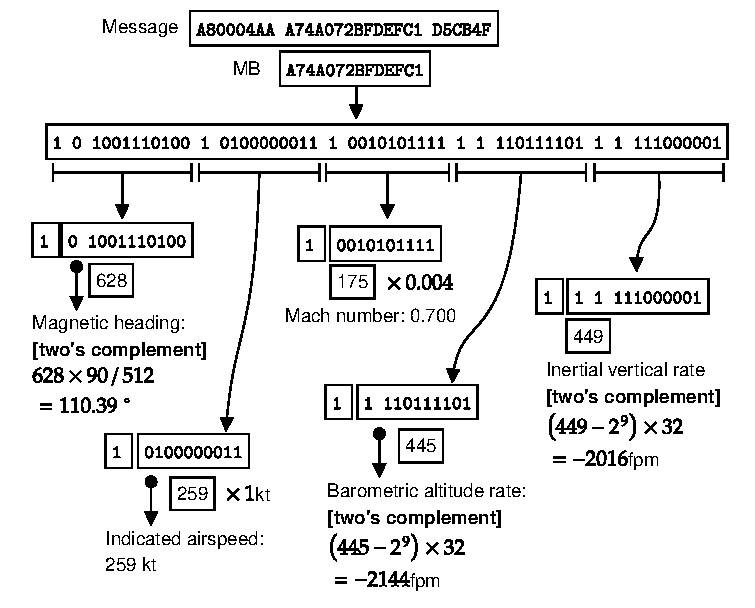
\includegraphics[scale=0.9]{figures/mode_s/bds60_example.pdf}
  \caption{BDS 6,0 decoding example}
  \label{fig:bds60_example}
\end{figure}

\begin{notebox}{Try it out}
Using pyModeS, we can decode information of BDS 6,0 messages as: 

\begin{verbatim}
import pyModeS as pms

msg = "A80004AAA74A072BFDEFC1D5CB4F"

pms.commb.hdg60(msg)      # 110.391, heading (deg)
pms.commb.ias60(msg)      # 259, ISA (kt)
pms.commb.mach60(msg)     # 0.7, Mach (-)
pms.commb.vr60baro(msg)   # -2144, baro vertical rate (ft/min)
pms.commb.vr60ins(msg)    # -2016, INS vertical rate (ft/min)
\end{verbatim}

\end{notebox}
